\section{Introduction}
\label{sec:intro}

\introepigraph
  {Treat things before they exist. Regulate things before disorder begins.}
  {Lao Tzu}
  {}

\noindent LLM-powered agents are becoming a common interface for complex work such as deep
research, coding, and tool-assisted question answering~\citep{IntroducingDeepResearch2025,
ManusHandsAI,ClaudeCodeClaude,GitHubCopilotYour2025,yao_react_2023,schick_toolformer_2024}.
In these systems, the LLM acts as the controller: it reasons over the user request,
emits a structured tool call, waits for the external tool to finish, and then resumes
generation using the tool result.
This \emph{Thought--Action--Observation} loop~\citep{yao_react_2023} is simple and safe,
but it is also often serial: each tool result conditions all subsequent tokens, so
the serving system cannot resume generation until the result arrives.
While the tool is running, the GPU often has no useful work to do for that agent turn.

This tool wait is hard to engineer away because it is structurally bounded by network
round-trips, container cold-starts, and database I/O that resist the exponential
improvements seen in model serving.
It is also large.
Our profiling across three benchmarks in Figure~\ref{fig:ttool_dist} shows that tool
execution accounts for 16--37\% of end-to-end wall time, and on turns with real network
tools the GPU is idle for the majority of the turn; \citet{sui_act_2026} report even
higher fractions, 35--61\% of total agent latency across agent workloads.

\begin{figure}[!t]
  \centering
  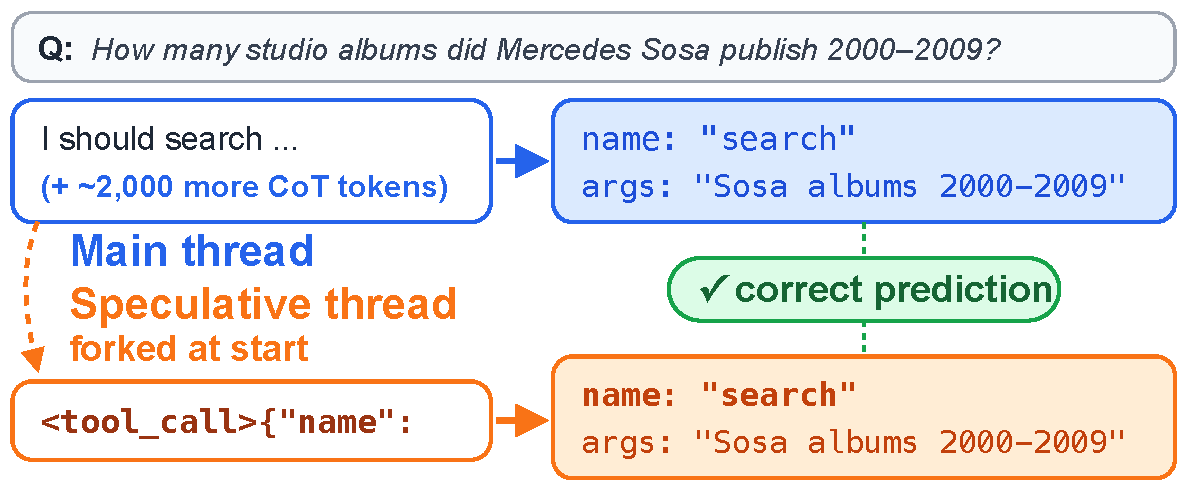
\includegraphics[width=0.92\columnwidth]{figures/fig_teaser_prompt.pdf}
  \caption{\textbf{Tool intent is visible early.}
  A speculative thread, forked at the main thread's first token with a forced tool-call
  prefix, predicts the exact tool call that the main thread emits ${\sim}2{,}000$ CoT
  tokens later.}
  \label{fig:teaser_prompt}
\end{figure}
\FloatBarrier



As LLM inference grows faster (through speculative decoding~\citep{leviathan_fast_2023},
hardware scaling, and disaggregated serving~\citep{zheng_sglang_2024}), the fraction of
wall time spent waiting for external tools \emph{increases}, not decreases, making
tool-wait the asymptotic bottleneck of agent latency.
Figure~\ref{fig:teaser_prompt} illustrates the opportunity this paper exploits: after a
single streaming token, a forked probe (sharing the same KV cache prefix) predicts the
identical web-search query that the main stream will emit after 2{,}000 tokens of
chain-of-thought.
The tool can be dispatched speculatively during those 2{,}000 tokens of decode, hiding
most of its network latency behind useful computation.

Existing systems attack adjacent parts of this problem but leave a gap for day-one,
\textit{training-free} deployment without predictors or historical traces.
Token-level speculative decoding~\citep{leviathan_fast_2023,li_eagle_2024,cai_medusa_2024}
and LLM serving systems~\citep{kwon_efficient_2023,zheng_sglang_2024,parrot24,
agrawal2024sarathiserve} reduce generation or serving overhead, but they do not dispatch
external tools earlier: the tool stall begins only \emph{after} the model has finished
emitting the call.
Workflow and serverless optimizers~\citep{orion,stojkovic2023specfaas,fu2024serverlessllm}
can prewarm or schedule known execution graphs, whereas tool-using agents generate their
next tool call online; there is no static graph to prefetch.

Recent agent-speculation systems move closer to execution-level overlap, but they rely on
a separate source of predictions: Speculative Actions~\citep{ye_speculative_2026} and
DualSpec~\citep{zhong_dualspec_2026} use predictors or verifier policies, while
PASTE~\citep{sui_act_2026} mines recurring tool-call patterns from historical traces.
These designs are powerful when traces, predictors, or repeated workflows are available;
they do not speculate from the currently running model alone.

\begin{figure}[!t]
  \centering
  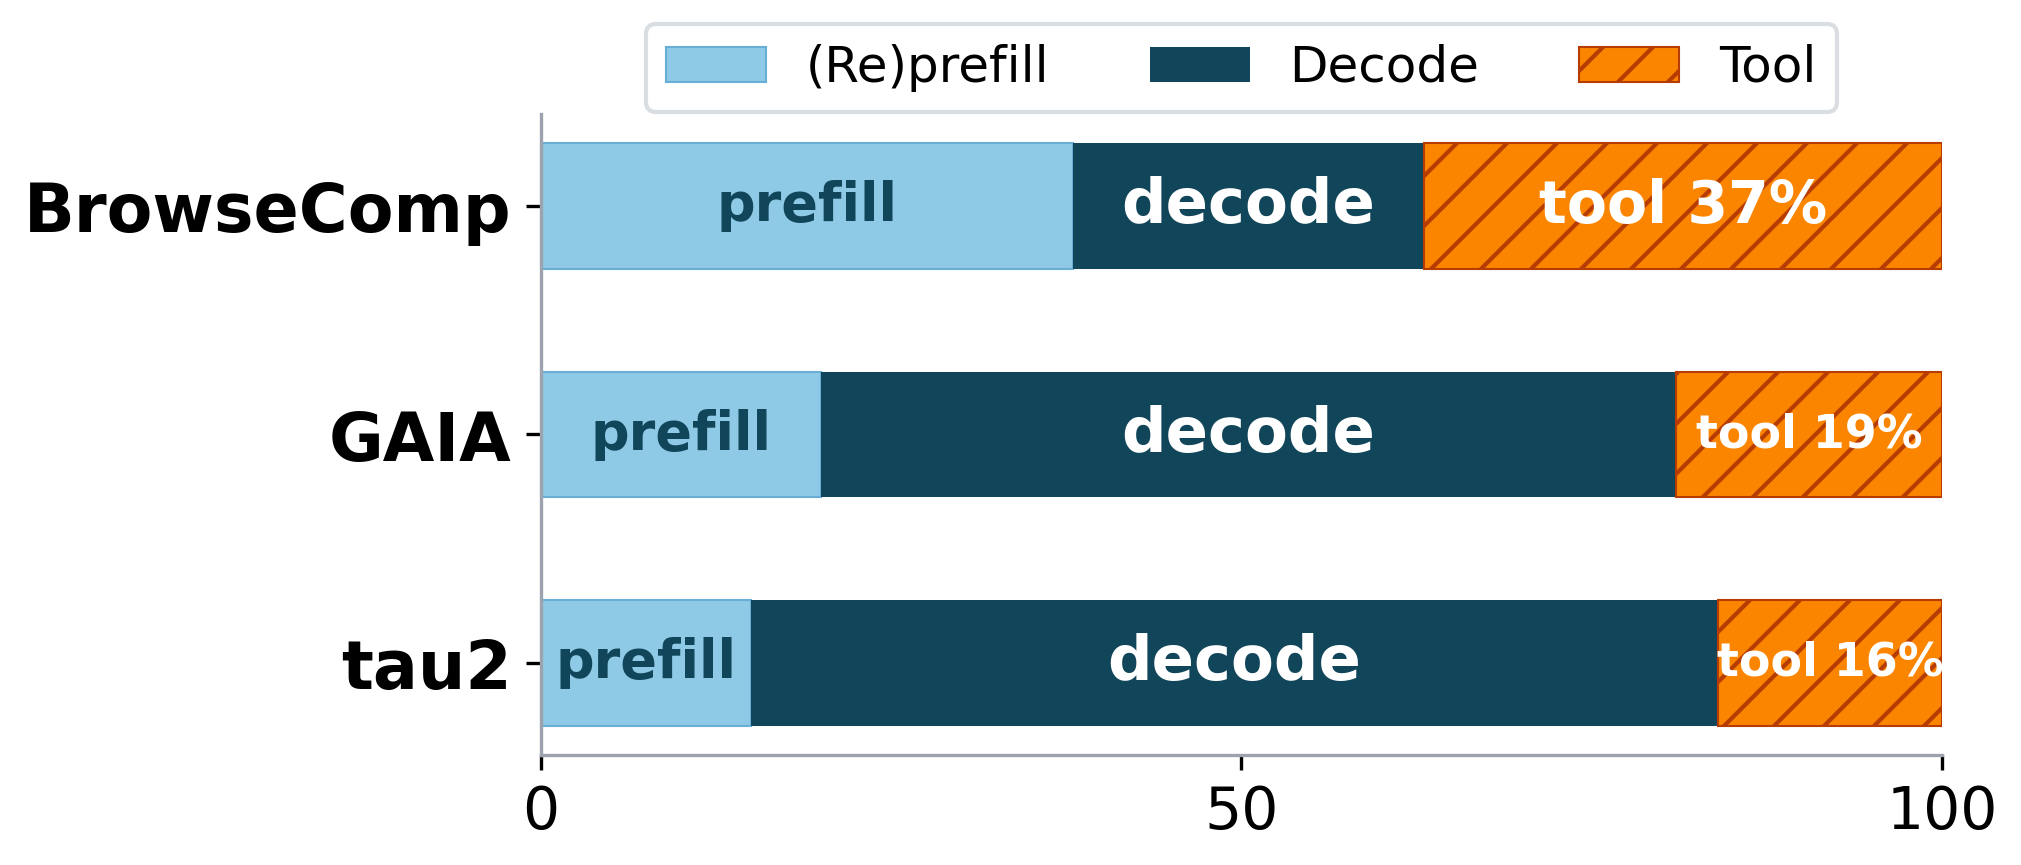
\includegraphics[width=0.92\columnwidth]{figures/fig1a_tool_fraction_bars.png}
  \caption{\textbf{Tool time is significant across agent tasks.} Across search, browsing, and database-style tasks, tool execution accounts for 16--37\% of end-to-end wall time.} %
  \label{fig:ttool_dist}
\end{figure}

The analogy to speculative execution in microprocessors is instructive: a CPU executes
past an unresolved branch and rolls back on misprediction.
The difference is the prediction source: where CPUs use branch predictors trained on
instruction history, \spork{} uses the running model itself, with no auxiliary model,
no trace collection, and no retraining.

\spork{} exploits a different opportunity: instruction-tuned models often reveal their
next tool call before completing the full chain-of-thought (\S\ref{sec:insight1}).
The fork also emits logprobabilities that indicate prediction confidence, and even failed
probes share a verified prefix with the final tool call.
These properties let the serving system turn the target model into its own speculative
tool predictor.

In this paper, we establish three empirical insights that make self-speculative tool use
viable.
First, Qwen3-32B~\citep{yang_qwen3_2025} predicts its own next tool call with high name accuracy (74.6--99.6\%
across GAIA~\citep{mialon_gaia_2024}, tau2-bench~\citep{barres_tau2_2025},
BrowseComp~\citep{wei_browsecomp_2025}, HotpotQA~\citep{yang_hotpotqa_2018}, and
BFCL~\citep{patil_bfcl_2025}) at the first-token fork point; the model already
``knows'' what it will do before finishing its reasoning (\S3.1).
Second, the probe's logprobability confidence separates correct from incorrect predictions
(0.90 vs.\ 0.46 mean span probability on GAIA), and argument accuracy climbs from 7.6\% to
97.5\% as more chain-of-thought context is observed (\S3.2).
Third, even when strict matching rejects a probe, the probe shares a median of 18 verified
tokens with the final tool call. Reused as a speculative-decoding \emph{draft}, these
tokens let the main stream skip re-decoding 35--50\% of the tool-call body (\S3.3).

\spork{} realizes this opportunity as a training-free controller for GPU-served tool
agents.
At each agent turn it \textbf{forks} the KV cache after the main generation's first token
(\textbf{D1}: near-zero overhead via prefix-cache sharing, reducing probe cost from 1.6\,s
to 0.35\,s), \textbf{gates} speculative dispatch on the probe's own logprob confidence
(\textbf{D2}: maximizes the accepted overlap by committing at the earliest confident
probe), and \textbf{recovers} verified prefix tokens from rejected probes via
speculative-decoding verification (\textbf{D3}: a median of 18 tokens recycled as drafts,
avoiding $\sim$0.6\,s of re-decode per rejected turn in offline analysis).
On a strict name-and-arguments match, \spork{} uses the pre-computed tool result;
otherwise it falls back to serial execution with no correctness penalty.

On GAIA (N=165, real web search, Qwen3-32B), the full \spork{} configuration (D1+D2+D3)
reduces median per-query latency by 10\% (P50: 34.7\,s $\to$ 31.2\,s) and tail latency by
18\% (P95: 131.9\,s $\to$ 108.1\,s) while preserving task accuracy (EM within 1\,pp of
baseline).
On HotpotQA (N=200, real Wikipedia API, Qwen3-32B), the full D1+D2+D3 configuration is
Pareto dominant: faster \emph{and} higher quality than the baseline simultaneously (P95
speedup 1.06$\times$, EM +1.5\,pp).
A latency sweep on tau2-bench (airline domain, N=43, simulated tool latency 0.5--5\,s) validates
the cost model: mean speedup grows monotonically with tool duration, from 1.09$\times$ at
a 0.5\,s tool floor to 1.18$\times$ at 5\,s, matching EQ1's prediction within 2\%.
The mechanism generalizes across model scale and architecture: it holds on Qwen3-4B (on
tau2; neutral elsewhere) and on
the Qwen3.5-35B-A3B~\citep{qwen_qwen35_2026} mixture-of-experts (16--20\% $P_{95}$ reduction across tau2, GAIA, and HotpotQA).
We also characterize when \spork{} does \emph{not} help: without thinking-mode
chain-of-thought the overlap window vanishes, and a model whose forced probe diverges
from its own tool-call format defeats self-speculation (\S6).

This paper makes the following contributions:
\begin{enumerate}
\item \textbf{Empirical insights (\S3).}
We show that Qwen3-32B predicts its own tool names with high accuracy (74.6--99.6\%) at the
fork point, exposes confidence through logprobabilities, and leaves
recoverable prefixes when strict matching rejects; we formalize the conditions under
which speculation breaks even via a cost model (EQ1, \S2.2).
\item \textbf{Training-free system design (\S4).}
We present three mechanisms (D1--D3) that realize speculative overlap within the standard
vLLM serving stack ($<$0.3\% TPOT overhead), requiring no model changes, no auxiliary
predictors, and no historical traces.
\item \textbf{End-to-end evaluation with real tools (\S6).}
On GAIA and HotpotQA with real network tools, \spork{} reduces $P_{95}$ latency by 6--18\%
while improving or preserving task accuracy, and the mechanism generalizes across
architecture (dense and MoE), with gains tapering to neutral at 4B scale on real-tool
benchmarks.
We validate the cost model against measured operating points and characterize when
speculation wins and when it does not.
\end{enumerate}
